\section{Introduction}\label{sec:intro}
A physics system is always described by an \emph{action functional} $S$ (if existed), possibly with some gauge symmetry,
\bea
S: \cE \to \bR,
\eea
where $\cE$ is the \emph{space of fields}. The classical physics is described by the \emph{critical locus} of the action functional, modulo gauge,
\bea
\on{Crit}(S)= \lcb \delta S=0\rcb / \sim.
\eea
$\delta S=0$ is called the \emph{equation of motion} which arises from the variation of the action functional $S$. 
In this lecture, we will focus on the quantum physics. One canonical way to approach the quantum physics is by the {\bf Feynman path integral},
\bea
\int_\cE \cO e^{iS/\hbar}.
\eea
$\cO$ is a function on $\cE$, called the (\emph{quantum}) \emph{observable}. When $\hbar$ is very small, the above integral
is asymptotically approximated around the critical locus of $S$; this is a method
called the \emph{stationary phase approximation}. The classical limit is obtained by $\hbar\to 0$.

Here are some typical examples of quantum field theory.
\bi[(1)]
\item \textbf{Scalar field theory}. $\cE=C^\infty(X)$. The fields are smooth functions on a manifold $X$.
\bea
S\lsb \phi\rsb = \int_X |d\phi|^2+m^2\phi^2, \quad \phi\in C^\infty(X).
\eea

\item \textbf{Gauge theory}. $\cE=\lcb \text{connections on } V\to X \rcb$. The fields are connections on a vector bundle $V\to X$ over $X$.
\bea
\text{Yang-Mills theory:  } \on{YM}[A] &=\int \Tr F\wedge \ast F, \quad F=dA+\hf [A,A].\\
\text{Chern-Simons theory:  } \on{CS}[A] &=\hf\int \Tr A\wedge dA+\frac{1}{6}\int \Tr A\wedge [A,A].
\eea
The Chern-Simons theory is described in 3 dimensions, $\on{dim} X=3$.

\item \textbf{Sigma model}. $\cE=\lcb \text{maps } (\Sigma \to X)\rcb$. The fields are maps between two manifolds.

\item \textbf{Gravity}. $\cE=\lcb \text{metrics on } X\rcb$. The fields are metrics on a manifold $X$.
\ei

In all the above examples, the space $\cE$ is HUGE in which the path integral are infinite-dimensional, $\int_\cE (\infty-\text{dim})$. 
In light of this fact, there are (mathematically) no rigorous definitions of the integrals in general.
This causes a big trouble in mathematics
to understand quantum physics.
However, in a special region such as the $\hbar$-asymptotic region (i.e. the asymptotic expansion as $\hbar\to 0$ around the critical points of $S$), the theory can usually be understood rigorously, giving rise to the \textbf{perturbative renormalization theory}. 
%This is a first approximation method and is far from understanding the full path integral; the latter is therefore called \emph{nonperturbative}. However, the approximation becomes exact in certain supersymmetric theories. 

\subsection{Observables}
Suppose we consider a quantum field theory (QFT) on a spacetime manifold $X$, and $\cE$ is the space of sections of a vector bundle $E$, denoted $\cE=\Gamma(X,E)$. We want to understand the integral $\int_\cE$.
\begin{itemize}
\item When $X=\text{point}$, $E=$ vector space, say, $\bR^n$, $\cE=\bR^n$. Hence,
$\int_\cE$ leads to the usual calculus that we learned in high school.

\item When $\on{dim} X>0$ (i.e. $X$ is not a point) and there is a fiber $E_p$ (for example, a linear space) at each point $p\in X$. But $\cE\neq \coprod_{p\in X} E_p$; the topology of $X$ makes a difference! This leads to some new algebraic structures, known as the \textbf{observable algebras}.
\bea 
\tikzset{every picture/.style={line width=0.75pt}}        
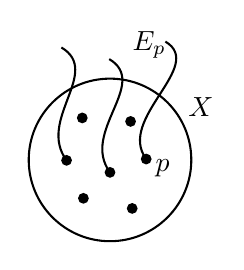
\begin{tikzpicture}[x=0.75pt,y=0.75pt,yscale=-1,xscale=1]

%Shape: Ellipse [id:dp02661356198166054] 
\draw   (175.17,106.61) .. controls (175.17,84.98) and (192.7,67.45) .. (214.33,67.45) .. controls (235.96,67.45) and (253.5,84.98) .. (253.5,106.61) .. controls (253.5,128.24) and (235.96,145.78) .. (214.33,145.78) .. controls (192.7,145.78) and (175.17,128.24) .. (175.17,106.61) -- cycle ;
%Shape: Ellipse [id:dp00618917520895268] 
\draw  [fill={rgb, 255:red, 0; green, 0; blue, 0 }  ,fill opacity=1 ] (198.91,86.38) .. controls (198.91,85.24) and (199.83,84.32) .. (200.97,84.32) .. controls (202.11,84.32) and (203.03,85.24) .. (203.03,86.38) .. controls (203.03,87.52) and (202.11,88.44) .. (200.97,88.44) .. controls (199.83,88.44) and (198.91,87.52) .. (198.91,86.38) -- cycle ;
%Shape: Ellipse [id:dp4985286560152604] 
\draw  [fill={rgb, 255:red, 0; green, 0; blue, 0 }  ,fill opacity=1 ] (191.34,106.82) .. controls (191.34,105.69) and (192.26,104.76) .. (193.4,104.76) .. controls (194.54,104.76) and (195.46,105.69) .. (195.46,106.82) .. controls (195.46,107.96) and (194.54,108.89) .. (193.4,108.89) .. controls (192.26,108.89) and (191.34,107.96) .. (191.34,106.82) -- cycle ;
%Shape: Ellipse [id:dp8690346263253921] 
\draw  [fill={rgb, 255:red, 0; green, 0; blue, 0 }  ,fill opacity=1 ] (222.19,88.07) .. controls (222.19,86.93) and (223.11,86) .. (224.25,86) .. controls (225.39,86) and (226.31,86.93) .. (226.31,88.07) .. controls (226.31,89.2) and (225.39,90.13) .. (224.25,90.13) .. controls (223.11,90.13) and (222.19,89.2) .. (222.19,88.07) -- cycle ;
%Shape: Ellipse [id:dp20263845603499497] 
\draw  [fill={rgb, 255:red, 0; green, 0; blue, 0 }  ,fill opacity=1 ] (212.27,112.61) .. controls (212.27,111.47) and (213.19,110.55) .. (214.33,110.55) .. controls (215.47,110.55) and (216.39,111.47) .. (216.39,112.61) .. controls (216.39,113.75) and (215.47,114.67) .. (214.33,114.67) .. controls (213.19,114.67) and (212.27,113.75) .. (212.27,112.61) -- cycle ;
%Shape: Ellipse [id:dp9834086999067779] 
\draw  [fill={rgb, 255:red, 0; green, 0; blue, 0 }  ,fill opacity=1 ] (229.71,106.19) .. controls (229.71,105.05) and (230.63,104.13) .. (231.77,104.13) .. controls (232.91,104.13) and (233.83,105.05) .. (233.83,106.19) .. controls (233.83,107.33) and (232.91,108.25) .. (231.77,108.25) .. controls (230.63,108.25) and (229.71,107.33) .. (229.71,106.19) -- cycle ;
%Shape: Ellipse [id:dp22592961134490075] 
\draw  [fill={rgb, 255:red, 0; green, 0; blue, 0 }  ,fill opacity=1 ] (199.46,125.11) .. controls (199.46,123.97) and (200.38,123.05) .. (201.52,123.05) .. controls (202.66,123.05) and (203.58,123.97) .. (203.58,125.11) .. controls (203.58,126.25) and (202.66,127.17) .. (201.52,127.17) .. controls (200.38,127.17) and (199.46,126.25) .. (199.46,125.11) -- cycle ;
%Shape: Ellipse [id:dp09074720791053226] 
\draw  [fill={rgb, 255:red, 0; green, 0; blue, 0 }  ,fill opacity=1 ] (222.96,129.98) .. controls (222.96,128.84) and (223.89,127.92) .. (225.03,127.92) .. controls (226.16,127.92) and (227.09,128.84) .. (227.09,129.98) .. controls (227.09,131.12) and (226.16,132.04) .. (225.03,132.04) .. controls (223.89,132.04) and (222.96,131.12) .. (222.96,129.98) -- cycle ;
%Curve Lines [id:da9825824283034781] 
\draw    (190.93,52.44) .. controls (210.59,64.17) and (178.97,87.32) .. (193.4,106.82) ;
%Curve Lines [id:da5263572037731432] 
\draw    (213.96,58.03) .. controls (233.62,69.77) and (199.9,93.11) .. (214.33,112.61) ;
%Curve Lines [id:da6829537734588929] 
\draw    (241.03,49.61) .. controls (260.69,61.34) and (217.34,86.69) .. (231.77,106.19) ;

% Text Node
\draw (223.77,43.4) node [anchor=north west][inner sep=0.75pt]    {$E_{p}$};
% Text Node
\draw (250.62,75.18) node [anchor=north west][inner sep=0.75pt]    {$X$};
% Text Node
\draw (234.77,105.03) node [anchor=north west][inner sep=0.75pt]    {$p$};
\end{tikzpicture}
\eea
\end{itemize}

Roughly speaking, 
\textbf{observables} are functions on fields (or certain homology), in which their space is denoted
$\sO(\cE)$. For example, 
distributions are \emph{linear observables}.
The new structures come from the following facts.
\begin{itemize}
\item Given an open subset $U\subset X$, we can talk about
\bea \on{Obs}(U)= \text{observables supported in } U.\eea

\begin{eg}
$\cE=C^\infty(X),\ p\in X$. Consider 
\bea \cO_1: \cE \to \bR,\eea
where $\cO_1(f)=f(p)^m, \ \forall f\in \cE$. $\cO_1$ is an observable supported in any open neighborhood of $p$.
\end{eg}

\item Let $\cE(U)=\Gamma(U,E)$. Then 
\bea
\on{Obs}(U)=\text{functions on }  \cE(U).
\eea

\item The new structure is the \textbf{factorization product / operator product expansion (OPE)}. Given disjoint open subsets $U_i \subset V$ contained in an open set $V$, such that the disjoint union is $\coprod_i U_i \subset V$, we have a map (factorization product) for observables:
\bea
\bigotimes_i \on{Obs}(U_i)\to \on{Obs}(V).
\eea

\item Intuitively, if $\cE(U)$ is restricted to $\cE(U_i)$, then dually $\sO(\cE(U_i))\to \sO(\cE(U))$.
Naively, we can \emph{multiply} those \emph{functions}, then we get
\bea
\bigotimes_i \on{Obs}(U_i)\to \on{Obs}(V).
\eea
This, however, requires further \emph{quantum corrections} in which fields in $U_i$'s may ``talk'' to each other.

\begin{eg}[Topological Quantum Mechanics (TQM)]
In topological QFT, $\on{Obs}(U)$ only depends on the topology of $U$.
Consider $\on{dim} X=1$ (a 1d QFT is a quantum mechanics) and $\on{Obs}(U)=A$ for any contractible open interval $U$. Now consider two open intervals $U_1$, $U_2$ on $X$ and embed them into a larger interval $V$.
\bea 
\tikzset{every picture/.style={line width=0.75pt}}         
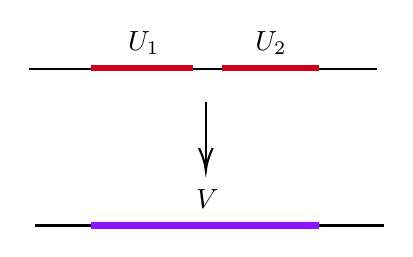
\begin{tikzpicture}[x=0.75pt,y=0.75pt,yscale=-1,xscale=1]


%Straight Lines [id:da49776176722773413] 
\draw    (470,30.46) -- (637.76,30.46) ;
%Straight Lines [id:da7522582205389852] 
\draw    (473.24,105.81) -- (641,105.81) ;
%Straight Lines [id:da9909036802138831] 
\draw    (555.34,46.5) -- (555.34,77.45) ;
\draw [shift={(555.34,79.45)}, rotate = 270] [color={rgb, 255:red, 0; green, 0; blue, 0 }  ][line width=0.75]    (10.93,-3.29) .. controls (6.95,-1.4) and (3.31,-0.3) .. (0,0) .. controls (3.31,0.3) and (6.95,1.4) .. (10.93,3.29)   ;
%Straight Lines [id:da11097180592386091] 
\draw [color={rgb, 255:red, 208; green, 2; blue, 27 }  ,draw opacity=1 ][line width=2.25]    (500,30) -- (549,30) ;
%Straight Lines [id:da6781384757672331] 
\draw [color={rgb, 255:red, 208; green, 2; blue, 27 }  ,draw opacity=1 ][line width=2.25]    (563,30) -- (610,30) ;
%Straight Lines [id:da2471941135880169] 
\draw [color={rgb, 255:red, 144; green, 19; blue, 254 }  ,draw opacity=1 ][line width=2.25]    (500,105.81) -- (610,105.81) ;

% Text Node
\draw (516.34,11) node [anchor=north west][inner sep=0.75pt]   [align=left] {$U_1$};
% Text Node
\draw (577.66,11) node [anchor=north west][inner sep=0.75pt]   [align=left] {$U_2$};
% Text Node
\draw (549.19,87.17) node [anchor=north west][inner sep=0.75pt]   [align=left] {$V$};
\end{tikzpicture}
\eea

We have a topological quantum mechanics (TQM) with maps
\bea
\on{Obs}(U_1)\otimes \on{Obs}(U_2) \to \on{Obs}(V) \quad \text{or} \quad A \otimes A \to A.
\eea
The factorization product does not depend on the location and size. We find an \textbf{associative algebra}!
\end{eg}
\end{itemize}


\paragraph{Algebraic structure.}
Consider two operators being placed at two different points on a line. When one operator approaches closely the other, the algebraic structure of the topology of the line comes from the homology group
\bea
H_{\blt} (\bR-\lcb 0\rcb)=H_0 (\bR-\lcb 0\rcb)= \bZ_{left} \oplus \bZ_{right}
\eea
which comprises the left and right multiplications.
\emph{Associativity} comes from a further consistency:
\bea &
\tikzset{every picture/.style={line width=0.75pt}}         
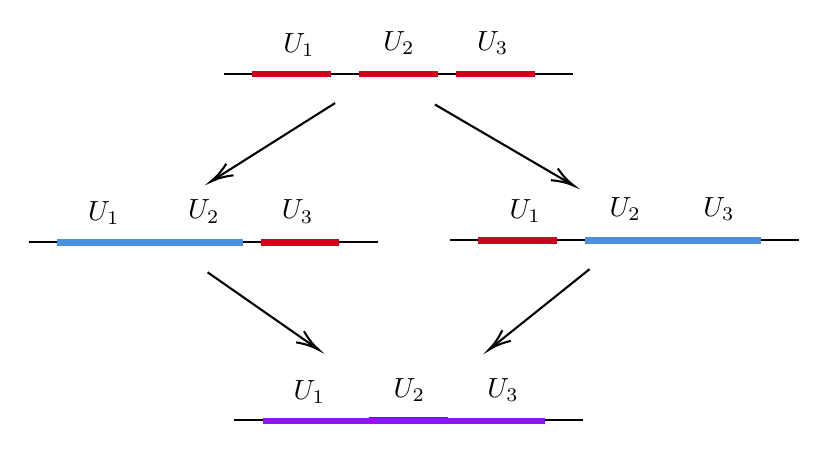
\begin{tikzpicture}[x=0.75pt,y=0.75pt,yscale=-1,xscale=1]
%Straight Lines [id:da5146107324067772] 
\draw    (162.3,64.67) -- (330.54,64.67) ;
%Straight Lines [id:da6366840570335301] 
\draw    (215.94,78.81) -- (157.69,115.6) ;
\draw [shift={(156,116.67)}, rotate = 327.73] [color={rgb, 255:red, 0; green, 0; blue, 0 }  ][line width=0.75]    (10.93,-3.29) .. controls (6.95,-1.4) and (3.31,-0.3) .. (0,0) .. controls (3.31,0.3) and (6.95,1.4) .. (10.93,3.29)   ;
%Straight Lines [id:da4584739157136033] 
\draw    (264,79.51) -- (329.27,117.66) ;
\draw [shift={(331,118.67)}, rotate = 210.3] [color={rgb, 255:red, 0; green, 0; blue, 0 }  ][line width=0.75]    (10.93,-3.29) .. controls (6.95,-1.4) and (3.31,-0.3) .. (0,0) .. controls (3.31,0.3) and (6.95,1.4) .. (10.93,3.29)   ;
%Straight Lines [id:da8016630535031757] 
\draw    (154.51,160.38) -- (206.36,196.52) ;
\draw [shift={(208,197.67)}, rotate = 214.88] [color={rgb, 255:red, 0; green, 0; blue, 0 }  ][line width=0.75]    (10.93,-3.29) .. controls (6.95,-1.4) and (3.31,-0.3) .. (0,0) .. controls (3.31,0.3) and (6.95,1.4) .. (10.93,3.29)   ;
%Straight Lines [id:da5351493584904696] 
\draw    (338.53,158.84) -- (291.56,196.42) ;
\draw [shift={(290,197.67)}, rotate = 321.33] [color={rgb, 255:red, 0; green, 0; blue, 0 }  ][line width=0.75]    (10.93,-3.29) .. controls (6.95,-1.4) and (3.31,-0.3) .. (0,0) .. controls (3.31,0.3) and (6.95,1.4) .. (10.93,3.29)   ;
%Straight Lines [id:da11490255972538899] 
\draw [color={rgb, 255:red, 208; green, 2; blue, 27 }  ,draw opacity=1 ][line width=2.25]    (176,65) -- (214,65) ;
%Straight Lines [id:da38887048079079545] 
\draw [color={rgb, 255:red, 208; green, 2; blue, 27 }  ,draw opacity=1 ][line width=2.25]    (227.42,64.67) -- (265.42,64.67) ;
%Straight Lines [id:da5815548933649641] 
\draw [color={rgb, 255:red, 208; green, 2; blue, 27 }  ,draw opacity=1 ][line width=2.25]    (274,65) -- (312,65) ;
%Straight Lines [id:da045018168844348505] 
\draw    (68.3,145.67) -- (236.54,145.67) ;
%Straight Lines [id:da9494212334866909] 
\draw [color={rgb, 255:red, 208; green, 2; blue, 27 }  ,draw opacity=1 ][line width=2.25]    (82,146) -- (120,146) ;
%Straight Lines [id:da13972709854409504] 
\draw [color={rgb, 255:red, 208; green, 2; blue, 27 }  ,draw opacity=1 ][line width=2.25]    (133.42,145.67) -- (171.42,145.67) ;
%Straight Lines [id:da49239786657156226] 
\draw [color={rgb, 255:red, 208; green, 2; blue, 27 }  ,draw opacity=1 ][line width=2.25]    (180,146) -- (218,146) ;
%Straight Lines [id:da018412058817521393] 
\draw    (271.3,144.67) -- (439.54,144.67) ;
%Straight Lines [id:da8371430474679855] 
\draw [color={rgb, 255:red, 208; green, 2; blue, 27 }  ,draw opacity=1 ][line width=2.25]    (285,145) -- (323,145) ;
%Straight Lines [id:da45745011041205896] 
\draw [color={rgb, 255:red, 208; green, 2; blue, 27 }  ,draw opacity=1 ][line width=2.25]    (336.42,144.67) -- (374.42,144.67) ;
%Straight Lines [id:da59402182478143] 
\draw [color={rgb, 255:red, 208; green, 2; blue, 27 }  ,draw opacity=1 ][line width=2.25]    (383,145) -- (421,145) ;
%Straight Lines [id:da3383677142840795] 
\draw    (167.3,231.67) -- (335.54,231.67) ;
%Straight Lines [id:da30399344382391535] 
\draw [color={rgb, 255:red, 208; green, 2; blue, 27 }  ,draw opacity=1 ][line width=2.25]    (181,232) -- (219,232) ;
%Straight Lines [id:da8362418177389068] 
\draw [color={rgb, 255:red, 208; green, 2; blue, 27 }  ,draw opacity=1 ][line width=2.25]    (232.42,231.67) -- (270.42,231.67) ;
%Straight Lines [id:da10310047941667388] 
\draw [color={rgb, 255:red, 208; green, 2; blue, 27 }  ,draw opacity=1 ][line width=2.25]    (279,232) -- (317,232) ;
%Straight Lines [id:da8603812711814927] 
\draw [color={rgb, 255:red, 74; green, 144; blue, 226 }  ,draw opacity=1 ][line width=2.25]    (82,146) -- (171.42,146) ;
%Straight Lines [id:da6924243205034588] 
\draw [color={rgb, 255:red, 74; green, 144; blue, 226 }  ,draw opacity=1 ][line width=2.25]    (336.42,145) -- (421,145) ;
%Straight Lines [id:da35290975414233494] 
\draw [color={rgb, 255:red, 144; green, 19; blue, 254 }  ,draw opacity=1 ][line width=2.25]    (181,232) -- (317,232) ;

% Text Node
\draw (189.46,43.85) node [anchor=north west][inner sep=0.75pt]   [align=left] {$U_1$};
% Text Node
\draw (237.64,43) node [anchor=north west][inner sep=0.75pt]   [align=left] {$U_2$};
% Text Node
\draw (282.83,43) node [anchor=north west][inner sep=0.75pt]   [align=left] {$U_3$};
% Text Node
\draw (95.46,124.85) node [anchor=north west][inner sep=0.75pt]   [align=left] {$U_1$};
% Text Node
\draw (143.64,124) node [anchor=north west][inner sep=0.75pt]   [align=left] {$U_2$};
% Text Node
\draw (188.83,124) node [anchor=north west][inner sep=0.75pt]   [align=left] {$U_3$};
% Text Node
\draw (298.46,123.85) node [anchor=north west][inner sep=0.75pt]   [align=left] {$U_1$};
% Text Node
\draw (346.64,123) node [anchor=north west][inner sep=0.75pt]   [align=left] {$U_2$};
% Text Node
\draw (391.83,123) node [anchor=north west][inner sep=0.75pt]   [align=left] {$U_3$};
% Text Node
\draw (194.46,210.85) node [anchor=north west][inner sep=0.75pt]   [align=left] {$U_1$};
% Text Node
\draw (242.64,210) node [anchor=north west][inner sep=0.75pt]   [align=left] {$U_2$};
% Text Node
\draw (287.83,210) node [anchor=north west][inner sep=0.75pt]   [align=left] {$U_3$};
\end{tikzpicture} \\ 
&\Longrightarrow (a\cdot b)\cdot c= a\cdot (b\cdot c),\quad a,b,c\in \text{Obs}(U_i),\ i=1,2,3.
\eea

\begin{eg}[Chiral QFT] Let $\on{dim }X=2$. The factorization product of a two-dimensional (2d) chiral theory is \textbf{holomorphic}.
\bea 
\tikzset{every picture/.style={line width=0.75pt}}     
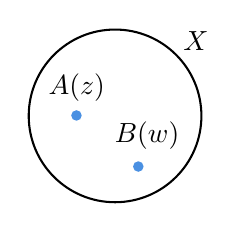
\begin{tikzpicture}[x=0.75pt,y=0.75pt,yscale=-1,xscale=1]

%Shape: Circle [id:dp46405244436709836] 
\draw  [color={rgb, 255:red, 74; green, 144; blue, 226 }  ,draw opacity=1 ][fill={rgb, 255:red, 74; green, 144; blue, 226 }  ,fill opacity=1 ] (144.8,123.47) .. controls (144.8,122.36) and (145.7,121.47) .. (146.8,121.47) .. controls (147.9,121.47) and (148.8,122.36) .. (148.8,123.47) .. controls (148.8,124.57) and (147.9,125.47) .. (146.8,125.47) .. controls (145.7,125.47) and (144.8,124.57) .. (144.8,123.47) -- cycle ;
%Shape: Ellipse [id:dp6198652930020687] 
\draw   (94,99.07) .. controls (94,76.09) and (112.62,57.47) .. (135.6,57.47) .. controls (158.58,57.47) and (177.2,76.09) .. (177.2,99.07) .. controls (177.2,122.04) and (158.58,140.67) .. (135.6,140.67) .. controls (112.62,140.67) and (94,122.04) .. (94,99.07) -- cycle ;
%Shape: Ellipse [id:dp42367483552549756] 
\draw  [color={rgb, 255:red, 74; green, 144; blue, 226 }  ,draw opacity=1 ][fill={rgb, 255:red, 74; green, 144; blue, 226 }  ,fill opacity=1 ] (115,98.87) .. controls (115,97.76) and (115.9,96.87) .. (117,96.87) .. controls (118.1,96.87) and (119,97.76) .. (119,98.87) .. controls (119,99.97) and (118.1,100.87) .. (117,100.87) .. controls (115.9,100.87) and (115,99.97) .. (115,98.87) -- cycle ;

% Text Node
\draw (102.06,77.07) node [anchor=north west][inner sep=0.75pt]    {$A( z)$};
% Text Node
\draw (134,100.27) node [anchor=north west][inner sep=0.75pt]    {$B( w)$};
% Text Node
\draw (167,57.07) node [anchor=north west][inner sep=0.75pt]    {$X$};
\end{tikzpicture}
\eea

\noindent In holomorphic coordinates, when an operator approach (or wind around) the other on $X$, the winding number can be kept track in terms of their Fourier/Laurent modes:
\bea 
A(z)B(w)=\sum_{n\in \bZ}\frac{\lb A_{(n)} B\rb (w)}{(z-w)^{n+1}}.
\eea
We find $\infty$-ly many ``products'' (or binary operations) $\lcb A_{(n)} B \rcb$. In this case, the observable algebra gives rise to a \textbf{vertex algebra}.
\end{eg}

Observable algebras are developed in the works of:
\begin{itemize}
    \item Beilinson-Drinfeld \cite{beilinson2004chiral}
    \begin{itemize}
        \item developed \textbf{factorization algebra} to formulate 2d chiral conformal field theory (CFT),
        \item introduced the notion of \textbf{chiral homology} (generalizing \emph{Hochschild homology} in one dimension).
    \end{itemize}
    \item Costello-Gwilliam \cite{costello2021factorization}
    \begin{itemize}
        \item constructed factorization algebras from perturbative renormalization theory, in the \textbf{Batalin-Vilkovisky (BV) formalism} \cite{BATALIN198127} (generalizing \emph{BRST formalism} in gauge theory).
    \end{itemize}
\end{itemize}

%\begin{rmk} The geometrical study of QFT are related to index theory: 1-dim. (Atiyah-Singer index theory), 2-dim. (chiral index theory on loop space). (see later) \end{rmk}

\subsection{BV formalism and homological integration}
Now we want to construct a homotopic renormalization in the perturbative BV formalism. The basic idea is formulated via the homological interpretation of integral, 
    \bea \boxed{\int \ =\ \text{homology}}\ .\eea
\paragraph{Calculus revisited.}
    Calculus is nicely packaged into the framework of de Rham theory. Let $M$ be a compact oriented manifold of $\on{dim} M=n$. Many constructions of integration on manifolds can be understood from de Rham complex
    $\lb \Omega^\blt(M), d\rb$, where $\Omega^\blt(M)$ is the space of smooth differential forms and $d$ is the de Rham differential. There is a natural integration map 
    \bea
    \int_M: \Omega^\blt(M) \to \bR,\quad
    \alpha\in \Omega^n(M) \mapsto \int_M \alpha\in \bR. \eea
    Observe that the $n$-th de Rham cohomology group
    $H^n_{dR}(M) =H^n\lb \Omega^\blt(M),d\rb\simeq\bR$. This implies that 
    \bea
    \int_M \ = \ H^n_{dR}. \eea
    The integration map is now
    \bea
    \Omega^n(M) \to H^n_{dR}(M),\quad
    \alpha \mapsto [\alpha].
    \eea
    This means that we can learn calculus by the algebraic structure on de Rham complex, even we do not know anything about measure theory. However, there is a problem of understanding $H^n_{dR}(M)$ when $n\to\infty$ as in QFT.
    
\paragraph{BV approach.}
    Define \textbf{polyvector fields}
    \bea 
    \on{PV}^\blt(M) =\bigoplus_k \on{PV}^k(M)\coloneqq \bigoplus_k \Gamma \lb M,\ \asym^k TM\rb.
     \eea
    Let $\Omega$ be a fixed volume form on $M$. We can naturally identify
    \bea
    \on{PV}^k(M) \xleftrightarrow{\ \lrcorner \Omega\ } \Omega ^{n-k}(M),\quad
    \mu\in \on{PV}^k(M) \lra \mu \lrcorner \Omega.
    \eea
    Locally, if $\Omega=e^\varphi dx^1\wedge \cdots \wedge dx^n$, $\mu=\mu^{i_1\cdots i_k} \partial_{i_1}\wedge \cdots \wedge \partial_{i_k}$, then
    \bea \mu \lrcorner\Omega= \sum \pm \mu^{i_1\cdots i_k} e^\varphi dx^1 \wedge \cdots \wedge \widehat{dx^{i_1}}\wedge \cdots \wedge\widehat{dx^{i_k}} \wedge \cdots \wedge dx^n. \eea
    
    %%%%%%%%%%%%%%%%%%%%%%%%%%%%%%%%%%%%
    The identification above leads to 
    \bea
    \begin{tikzcd}
    \Omega^{0} \ar[r, "d"] \ar[dd, "\simeq"] 
    & \Omega^{1} \ar[r, "d"] \ar[dd, "\simeq"] 
    & \cdots \ar[r,"d"] & \Omega^{n} \ar[dr, "\int"] \ar[dd, "\simeq"] & \\
     & & & & \bR \\
    PV^{n} \ar[r, "\Delta"]
    & PV^{n-1} \ar[r, "\Delta"]
    & \cdots \ar[r, "\Delta"] & PV^{0}  \ar[ur, swap, "\int_{BV}"] & 
    \end{tikzcd}
    \eea
where
$\Delta: \on{PV}^k \to \on{PV}^{k-1}$ is a divergence operator with respect to $\Omega$. $\Delta$ is called the \textbf{BV operator}, induced from the de Rham differential operator $d$.
For example, 
$\Delta: \on{PV}^1=\on{Vect}(M) \to \on{PV}^0=C^\infty(M)$ is the usual divergence.

$\int_{BV}$ is the \textbf{BV integration}, which is a map
\bea \int_{BV}: \on{PV}^0 \to \bR,\quad 
f \mapsto \int f\Omega.
\eea
Homologically $\int_{BV}$ can be identified with $H^0_{BV}$, i.e. \bea \boxed{\int_{BV}= H^0}\ .\eea
Here ``$\on{dim} (M)$'' does not appear. The problem of integration is transferred to construct $\Delta$, which has a convenient formulation at least in perturbative QFT. This is one of the folklore advantage of working with BV.
The challenge now is to construct $\Delta$ in the $\infty$-dimensional setting.
In $\infty$ dimensions (as in QFT), renormalization helps to construct $\Delta$, leading to a \textbf{homological integration}.

\paragraph{Explicit form of $\Delta$.}
Locally in $U$, let $\lcb x_i\rcb_{i=1}^n$ be local coordinates and $\Omega=e^{f(x)}dx^1\wedge \cdots \wedge dx^n$ be the volume form. Introduce the vector fields $\partial_i=\frac{\partial}{\partial x_i}$, then the polyvector field is \bea \on{PV}(U)=C^\infty(U) [\partial_1, \cdots, \partial_n],\eea
where $\partial_i$'s are anticommuting: $\partial_i \partial_j =- \partial_j \partial_i$. 
Let us write $\theta_i=\partial_i$ (\textit{note}: this is a vector field, NOT an differential operator), then a local section $\mu\in \on{PV}(X)$ can be written as a function of $x^i$, $\theta_i$:
\bea
\mu=\mu (x^i, \theta_i)
\eea
with $x^ix^j=x^j x^i$ and $\theta_i \theta_j =- \theta_j \theta_i$.
Let $\frac{\partial}{\partial x^i}$ be the derivative with respect to $x^i$  and $\frac{\partial}{\partial \theta_i}$ be the derivative with respect to $\theta_i$ (from the left). Then the BV operator is given locally by 
\bea
\Delta = \sum_i \frac{\partial}{\partial x^i} \frac{\partial}{\partial \theta_i}
+\sum_i (\partial_i f) \frac{\partial}{\partial \theta_i}
\eea
which looks like a second order operator (it is easy to check that $\Delta^2=0$). This is in contrast with de Rham differential $d$, which is a first order differential
operator. Note that the first term looks like a Laplacian, but it is NOT. $\theta_i$ is an odd variable. Hence, $\Delta$ is sometimes called an \emph{odd Laplacian}.

\begin{eg}[$\frac{\partial}{\partial \theta_i}$ operator]
\bea\frac{\partial}{\partial \theta_1}(\theta_1\theta_2) &=\theta_2,\\
\frac{\partial}{\partial \theta_1}(\theta_2\theta_1) &=- \frac{\partial}{\partial \theta_1}(\theta_1\theta_2)=-\theta_2.
\eea
\end{eg}

\begin{eg}[Singularity theory: an example of $\int_{BV}$]
Consider the $n$-dimensional complex space $\bC^n$. Let $f(z^i): \bC^n\to \bC$ be a polynomial in $n$ variables with an isolated critical point at the origin, 0:
\bea \on{Crit}(f)=\lcb 0\rcb.\eea
We consider holomorphic/polynomial polyvector fields
\bea \cA =\bC[z^i, \theta_i], \quad
\theta_i \theta_j =- \theta_j \theta_i.\eea
Let the BV operator be
\bea \Delta=\hbar \sum_{i=1}^n \frac{\partial}{\partial z^i} \frac{\partial}{\partial \theta_i}
+\sum_i (\partial_i f) \frac{\partial}{\partial \theta_i}. \eea
\begin{itemize}
    \item $f(z^i)$ gives a solution of the quantum master equation (QME) in $\cA[[\hbar]]$: $\Delta f = \lcb f, f\rcb = 0$.
    \item The space of quantum observables, $\on{Obs}^q=H^\blt (\cA [[  \hbar]], \hbar\Delta+\lcb f,-\rcb)$, is isomorphic to a formal completion of the Brieskorn lattice \cite{saito1983higher}.
    \item 
    The quantum observable (or Brieskorn lattice) plays an important role of Hodge filtration (which is related to $\hbar$-filtration) in singularity theory (see \cite{arnold2012singularities,kulikov1998mixed} for an exposition).
    \item The BV-integration models the oscillatory integral 
    \bea \lan \cO\ran=\int_{\mathcal{L}} d^n z\ \cO e^{f/\hbar},\eea where $\mathcal{L}$ is a Lefschetz thimble.
    \item The above finite-dimensional model is the effective theory of topological Landau-Ginzburg B-model. 
    \item In general, a QFT can be viewed as a version of $\infty$-dimensional singularity theory.
\end{itemize}
\end{eg}

\noindent \textsc{Reference}: \cite{Li:2017exk}.
